
\newpage
\section{Applications to the Cahn Hilliard equation }%
\label{sec:cahn_hilliar_applications}

In this section, we will demonstrate that the proposed cut finite element method can be used to solve the Cahn-Hilliard problem. Firstly, we will recall the strong form and illustrate how it can be recast into a weak form following the approach in
\cite{feng2007fully}. Subsequently, we will derive a simplistic numerical time iteration scheme to demonstrate that the solution to the problem can indeed be found. Again, all numerical experiments are conducted using the open-source finite element method (FEM) framework, Gridap, as documented in \cite{verdugo22}.


\subsection{Deriving the discrete formulation of the Cahn-Hilliard equation}%
\label{sub:revisiting_the_strong_formulation}

 Recall the strong formulation of the Cahn-Hilliard equation.
Let $ u( x,0) =  u_{0}$ then is the dynamics on the form,
\begin{subequations}
\label{eq:strong_ch}
    \begin{align}
\partial _{t} u + \Delta  \left(  \varepsilon^2  \Delta u - f( u) \right)   &=0  \quad \text{ in } \Omega  \\
\partial _{n} u &= 0 \quad \text{ on } \Gamma  \\
\partial _{n}    \Delta u       &= 0 \quad \text{ on } \Gamma
    \end{align}
\end{subequations}
Here we define $f( u) = u( u^{2} -1)  = F' ( u)  $ where $F( u) = ( 1 / 4 ) ( u^2 -1 ) ^{2} $. With the corresponding energy. We define the small parameter to be $\varepsilon  = 1 / 100$.
\begin{equation}
    \label{eq:physical_prop}
E( u)  = \int_{\Omega }^{} \frac{\varepsilon^{2} }{2} \abs{ \nabla u } ^2 +  F( u) dx
\end{equation}

We also recall that the energy functional monotonically decreasing and that the global mass concentration is conserved, i.e.
\begin{equation}
\label{eq:mass_cons_energy_decrease2}
\frac{d}{dt} E( u)  <  0 \text{ and }\frac{d}{dt} \int_{\Omega }^{}  u dx = 0.
\end{equation}

For convenience, we decompose the functional so that $E(u) = E_{1}(u) + E_{2}(u)$. Here, $E_{1}(u) = \int_{\Omega } \frac{\varepsilon^{2}}{2} |\nabla u|^2 , dx$ represents the smoothing contribution, while $E_{2}(u) = \int_{\Omega } F(u) , dx$ represents the separation contribution.

Now assume that $u \in L^2( [0,T], H^{4}( \Omega ) ) $ and $v_{h} \in  V_{h}$ of order $k$. It is clear that the initial weak formulation is,
\begin{equation}
    ( \partial_{t} u,v_{h} )_{\Omega }  + \varepsilon^{2} ( \Delta ^2u, v_{h})_{\Omega } -  ( f( u), v_{h} )_{\Omega } = 0.
\end{equation}

As we can see did the biharmonic equation appear and, thus, we can apply the cut finite element framework developed in Section \ref{sec:cutcip_biharmonic_problem}. We define the discrete weak problem as follows.
\begin{equation}
    \begin{split}
        & \text{Find  }u_{h} \in L^{2}( [0,T],V_{h})  \text{ such that } \forall v_{h} \in V_{h} \\
        & ( \partial_{t} u_{h},v_{h} )_{\Omega }   + \varepsilon^{2} A_{h}( u_{h},v_{h})   +  c_{h}( u_{h},v_{h})  = 0.
    \end{split}
\end{equation}
Here we have followed the nonlinear weak formulation \cite[Equation
4.2]{feng2007fully} and the cut finite element bilinear form for the biharmonic equation proposed in Equation \eqref{eq:discrete_CutCIP_prob} such that
\begin{align}
    c_{h}( u_{h}, v_{h})  & = ( f( u_{h}) ,\Delta v_{h})_{\Omega } +  ( f( u_{h}) , \partial _{n}v)_{\mathcal{F}_{h} } \\
    A_{h}( u_{h}, v_{h})  & =  a_{h}( u_{h}, v_{h}) + g_{h}( u_{h}, v_{h})
\end{align}

The primary aim is to formulate demonstrate that this problem can be solved using a simple time-integration scheme. Define the index $m= 0, 1, \ldots, M$. This index corresponds to uniformly distributed time points $t_{m}$, which are subject to the
boundary conditions $t_{0} = 0$ and $t_{M} = M \tau$. Here, we denote the time step as $\tau = \varepsilon^2$. Each time step $u^{m}_{h}$ is an element of the discrete space $V_{h}$ , i.e. $u^{m}_{h} \in V_{h}$  with the initial condition defined as $u^{0} = u( t_{0},x )$. Following this, we establish the forward difference operator, which is determined by the time step $\tau $.
\begin{equation}
\overline{\partial } _{t} u_{h}^{m} = \frac{u_{h}^{m} - u_{h}^{m-1}}{ \tau }
\end{equation}

We define the Implicit explicit scheme (IMEX) scheme to have the following discretization,
\begin{equation}
( \overline{\partial } _{t} u^{m}_{h}, v_{h}   )_{\Omega } + \varepsilon^{2} A^{m}_{h}( u_{h}^{m} , v) +  c_{h} (  u_{h}^{m-1}, v_{h})  = 0 , \quad \forall v_{h}, u^{m}_{h} \in V^{}_{h}.
\end{equation}
which equivalently can be rewritten as
\begin{equation}
( u_{h}^{m},v )_{\Omega }  + \tau \varepsilon^{2} A_{h}( u_{h}^{m} , v)   =  ( u_{h}^{m-1},v )_{\Omega } - \tau c_{h} (  u_{h}^{m-1}, v) .
\end{equation}
Hence, we have a complete space time scheme.


\subsection{Demonstration on the Cahn-Hilliard problem}%
\label{sub:demonstration_on_the_physical_cahn_hilliard}

For the strong form of the Cahn-Hilliard \eqref{eq:strong_ch} we have no analytical solution, so we cannot construct a manufactured solution. However, a way to check that the system does behave like expected based on the physical properties \eqref{eq:physical_prop}. In other
words, we can check that our discrete solution satisfies the following conditions. We define the discrete values $E^m = E( u_{h}^{m})$, $E_{1}^m = E_{1}( u_{h}^{m})$ and $E_{2}^m = E_{2}( u_{h}^{m})$ and the initial function  $u_{0} = u( x,0) $. From
the physical properties \eqref{eq:physical_prop} to we expect the discrete equivalent to hold, i.e.
\begin{equation}
    E^m   <  E^{ m-1 } \text{ and }   \int_{\Omega }^{} u_{h}^{m}   dx \approx \int_{\Omega }^{} u_{0}  dx.
\end{equation}
To test this, we check that $ \delta E^{m} >0 $ generally holds, where
\begin{equation}
 \delta E^{m} = E( u_{h}^{m-1}) -  E( u_{h}^{m}) ,  \\
\end{equation}
 Similarly, let us define the relative cumulative global mass error and local mass error.
 \begin{equation}
 \Delta u_{h}^{m}  = \frac{ \abs{ \int_{\Omega }^{}  ( u_h^{m} - u_{0} ) dx } }{ \abs{ \int_{\Omega }^{}  u_{0} dx } } \quad \text{ and } \quad
 \delta u_{h}^{m}  = \frac{  \int_{\Omega }^{}  ( u_h^{m} - u^{m-1}_{h} ) dx  }{ \abs{ \int_{\Omega }^{}  u_{0} dx } }.
 \end{equation}
 To test mass conservation we expect the error $\Delta u_{h}^{m}$ and $\delta u_{h}^{m}$   to be close to zero.

\begin{figure}[]
    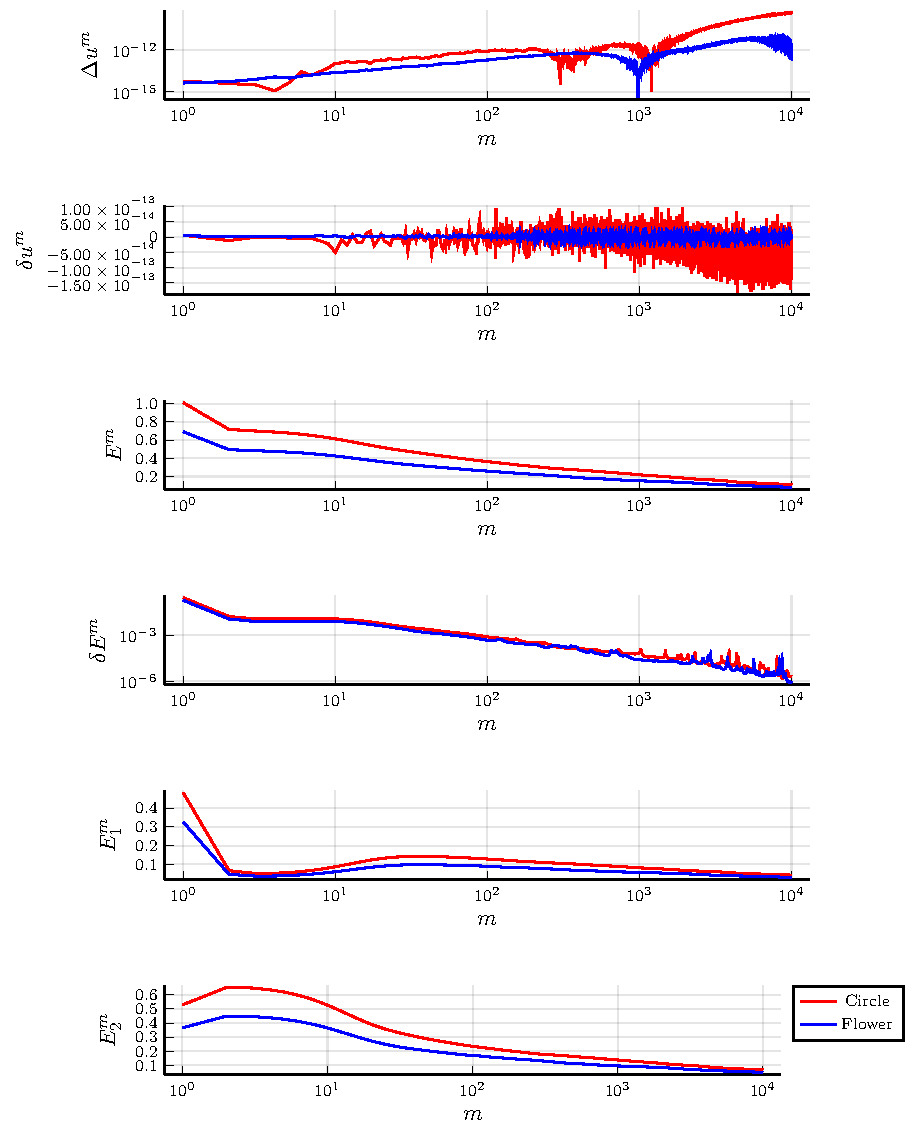
\includegraphics{results/physical_CH_plot.pdf}
    \caption{Evolution of the total discrete energy $E^m$ and the local energy difference $\delta E^m$, global mass conservation $\Delta u^m$, and the local mass difference $\delta u^m$ on a circular domain and a flower-shaped domain. }
    \label{fig:physical_CH_plot}
\end{figure}

\begin{figure}[]
    \centering
    \hfill
    \subfloat[$t=0\tau$]{
        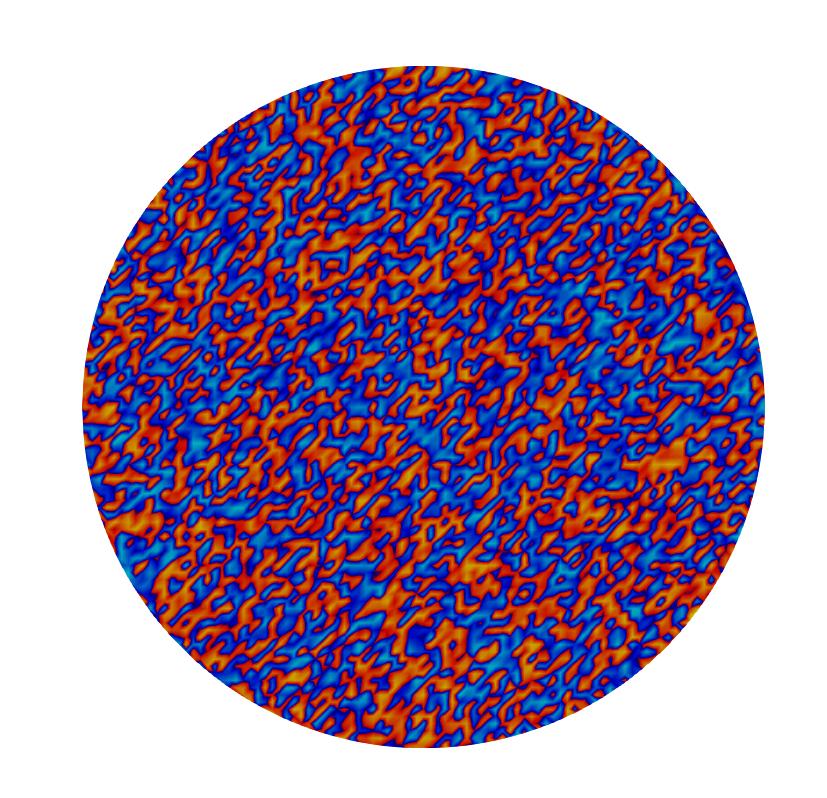
\includegraphics[width=0.3\textwidth]{results/illustration/c0.png}
    }\hfill
    \subfloat[$t=2\tau$]{
        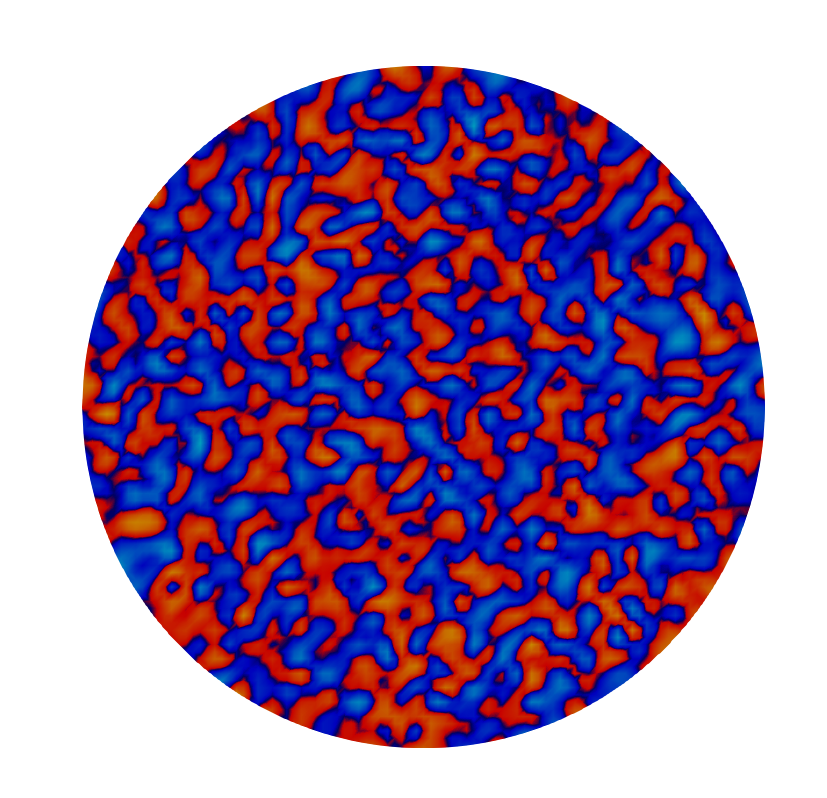
\includegraphics[width=0.3\textwidth]{results/illustration/c2.png}
    }
    \hfill
    \subfloat[$t=10\tau$]{
        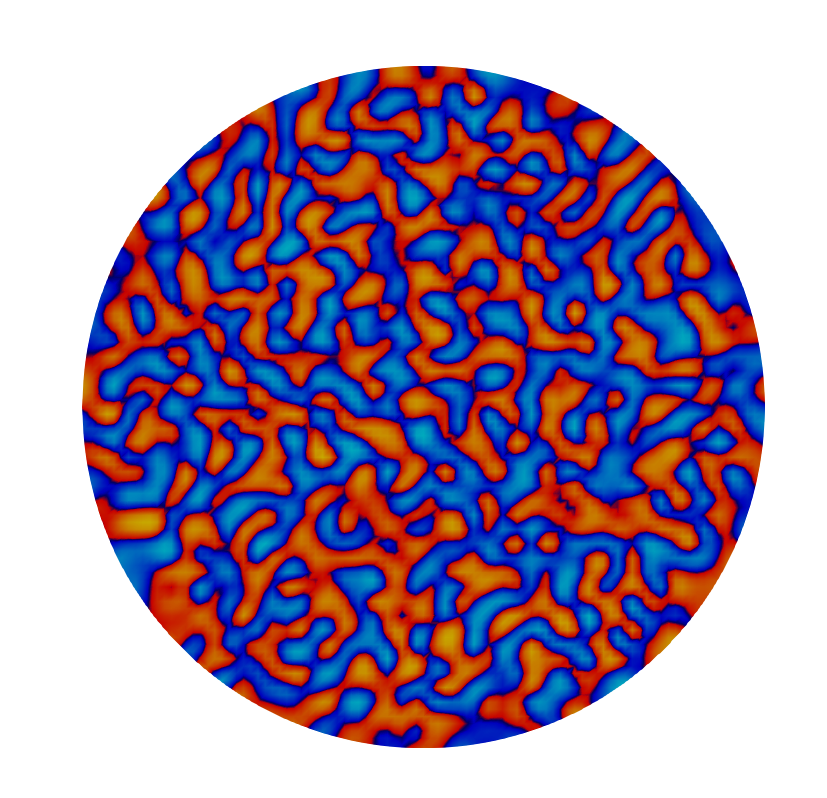
\includegraphics[width=0.3\textwidth]{results/illustration/c10.png}
    }
    \\
    \vspace{10pt}
    \hfill
    \subfloat[t=50$\tau$]{
        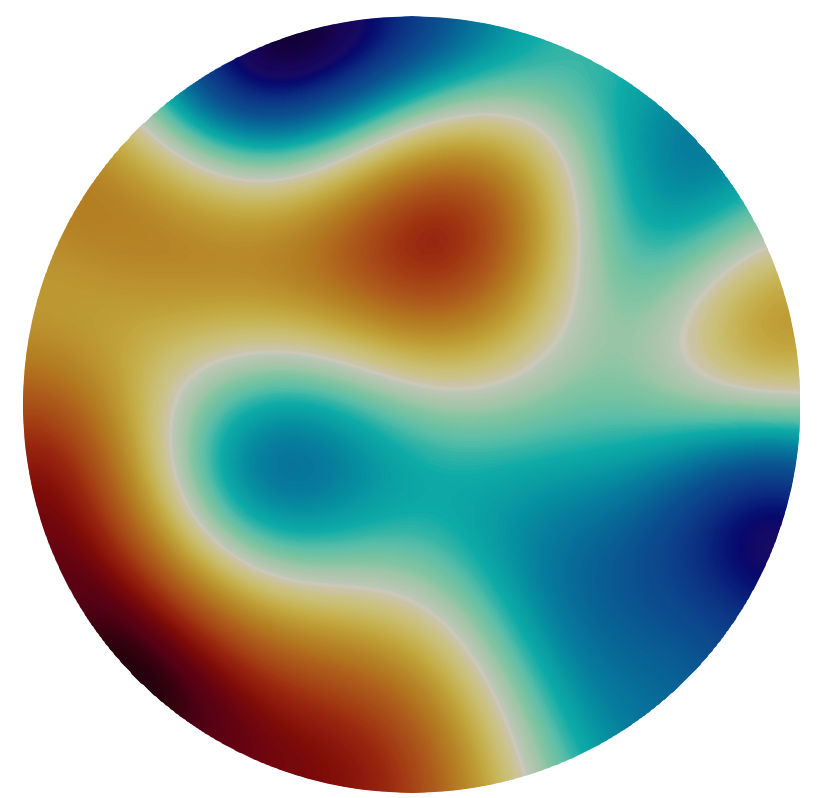
\includegraphics[width=0.3\textwidth]{results/illustration/c50.png}
    }
    \hfill
    \subfloat[$t=200\tau$]{
        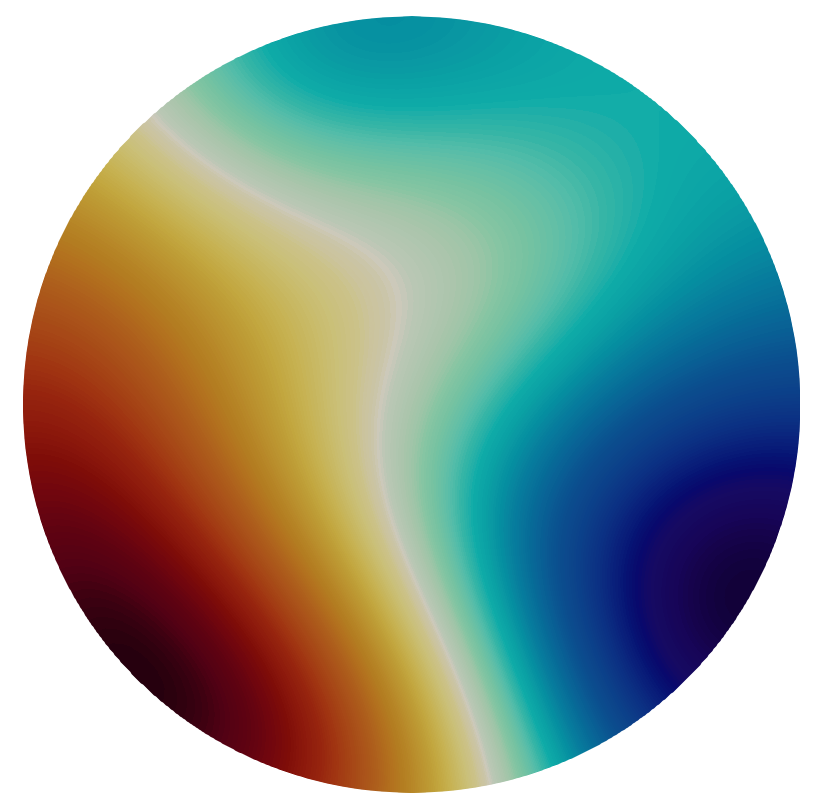
\includegraphics[width=0.3\textwidth]{results/illustration/c200.png}
    }\hfill
    \subfloat[$t=1000\tau$]{
        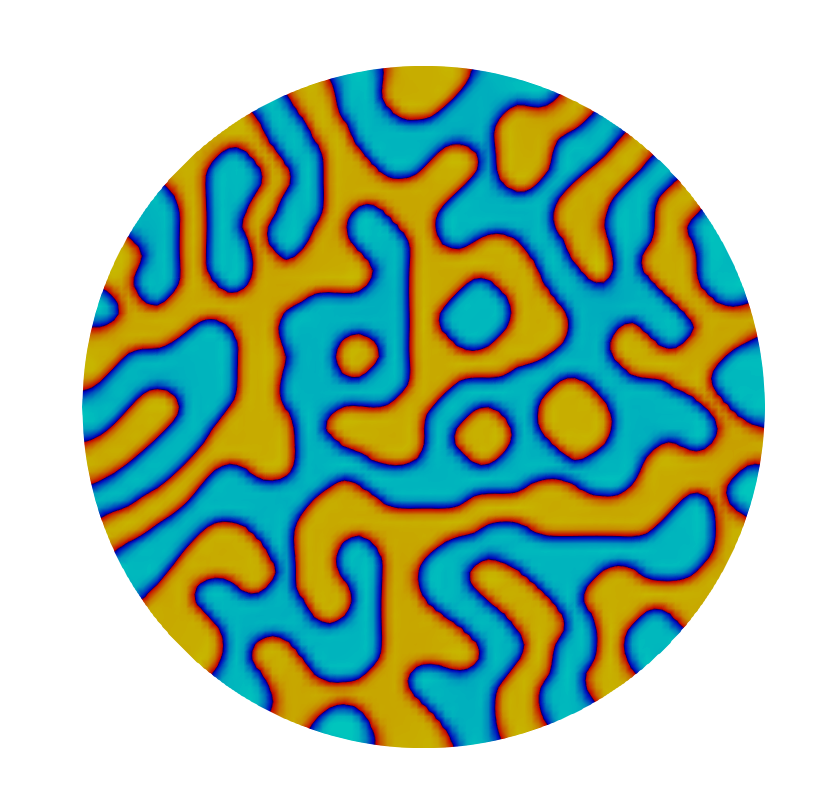
\includegraphics[width=0.3\textwidth]{results/illustration/c500.png}
    }
    \\
    \vspace{10pt}
    \hfill
    \subfloat[$t=50\tau$]{
        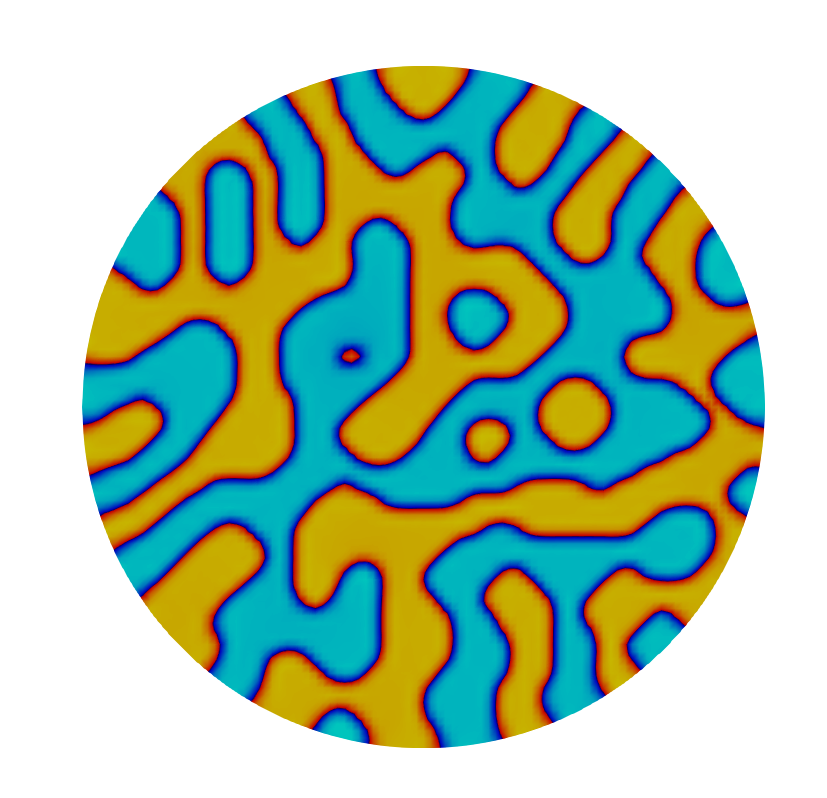
\includegraphics[width=0.3\textwidth]{results/illustration/c1000.png}
    }
    \hfill
    \subfloat[$t=200\tau$]{
        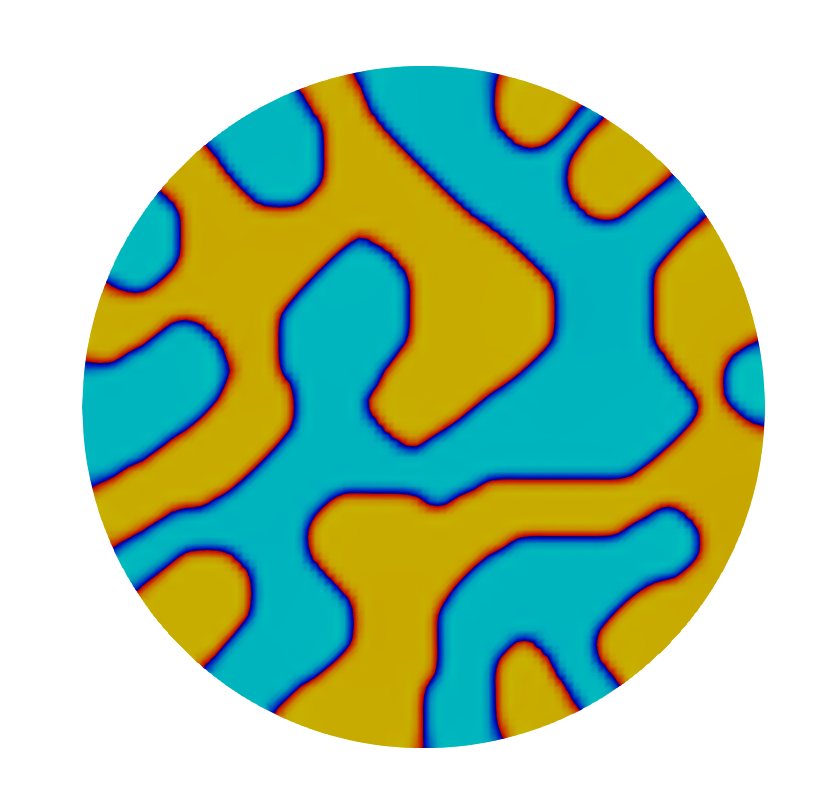
\includegraphics[width=0.3\textwidth]{results/illustration/c5000.png}
    }\hfill
    \subfloat[$t=1000\tau$]{
        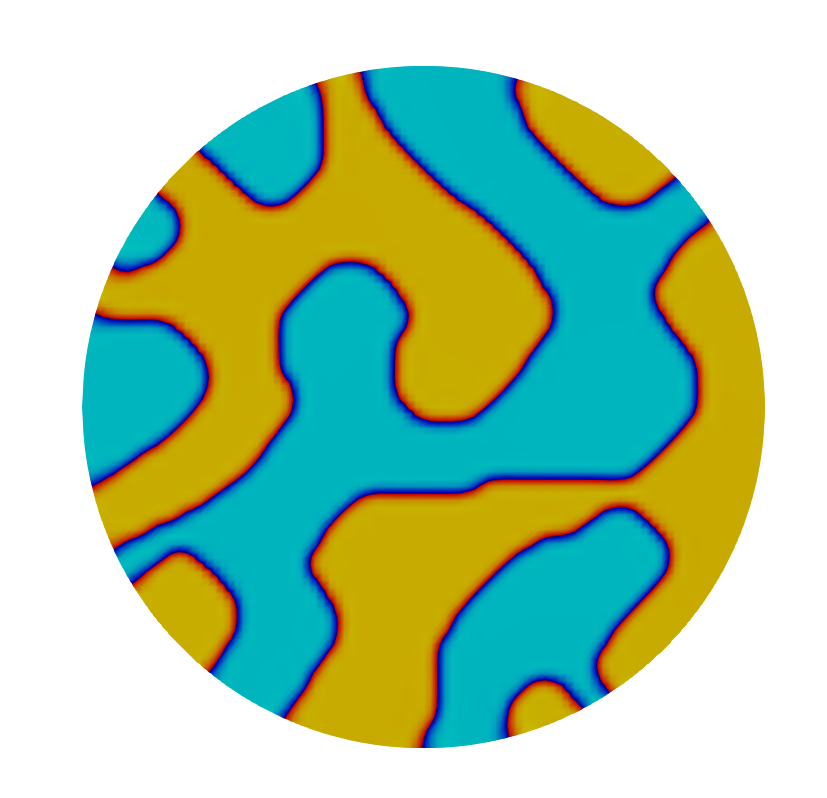
\includegraphics[width=0.3\textwidth]{results/illustration/c10000.png}
    }
    \vspace{10pt}
        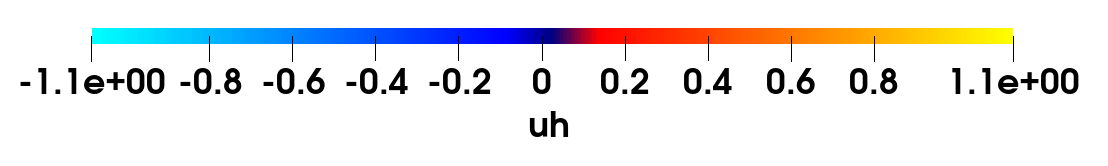
\includegraphics[width=0.8\textwidth]{results/illustration/colobar.png}

    \caption{Illustration of simulations of the Cahn-Hilliard equation on the circle domain for $t\in \left[ 0, 10000\tau  \right] $.}
        \label{sub:fig:ill_circle}
\end{figure}

\begin{figure}[]
    \centering
    \hfill
    \subfloat[$t=0\tau$]{
        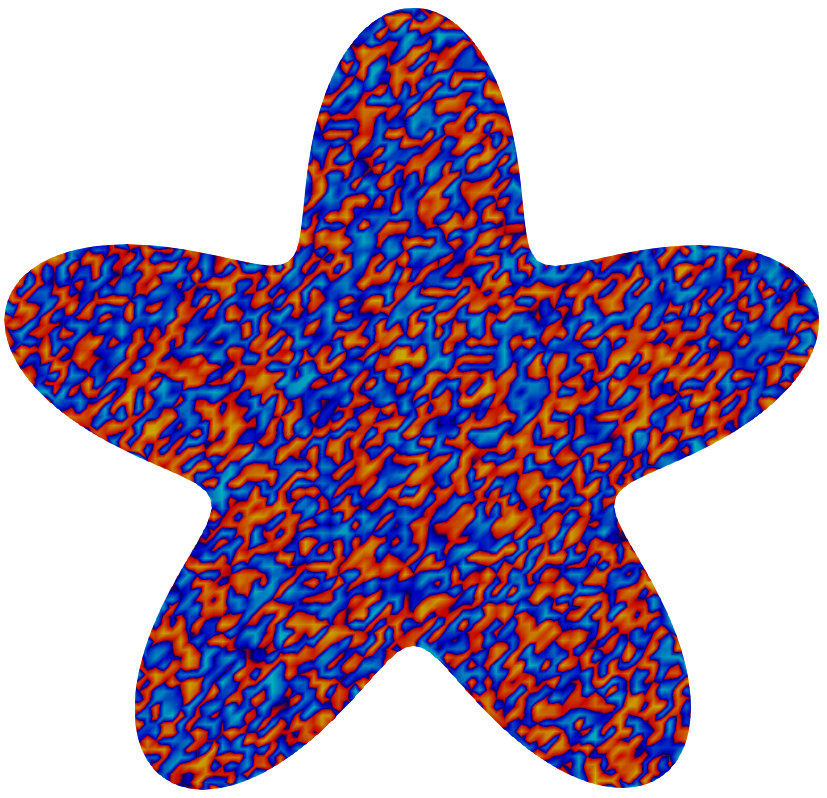
\includegraphics[width=0.3\textwidth]{results/illustration/f0.png}
    }\hfill
    \subfloat[$t=2\tau$]{
        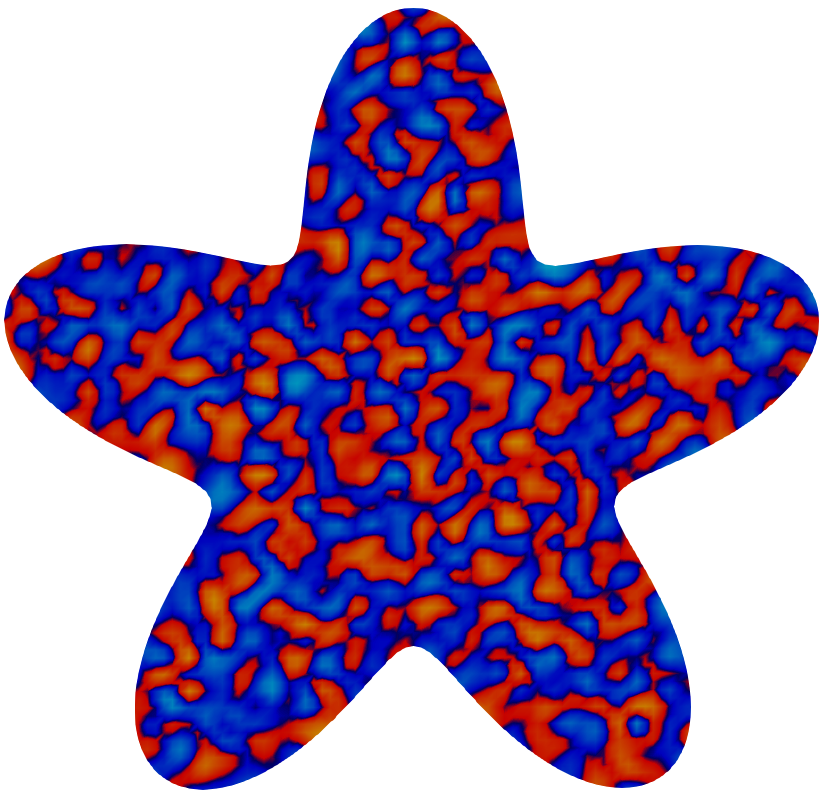
\includegraphics[width=0.3\textwidth]{results/illustration/f2.png}
    }
    \hfill
    \subfloat[$t=10\tau$]{
        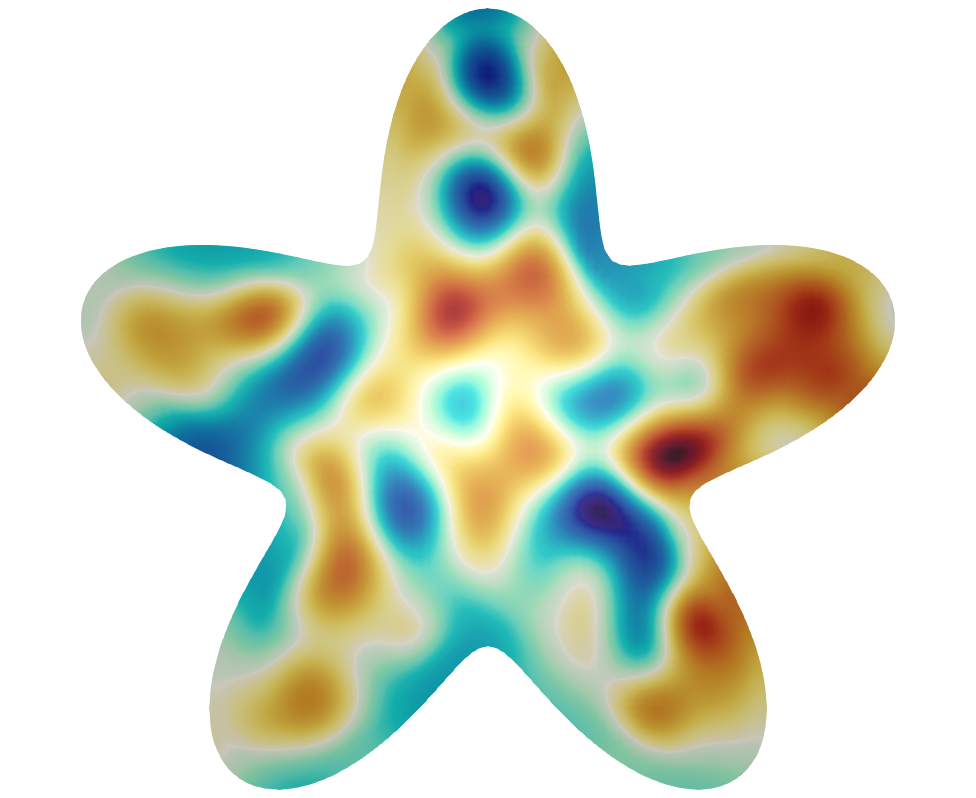
\includegraphics[width=0.3\textwidth]{results/illustration/f10.png}
    }
    \\
    \vspace{10pt}
    \hfill
    \subfloat[t=50$\tau$]{
        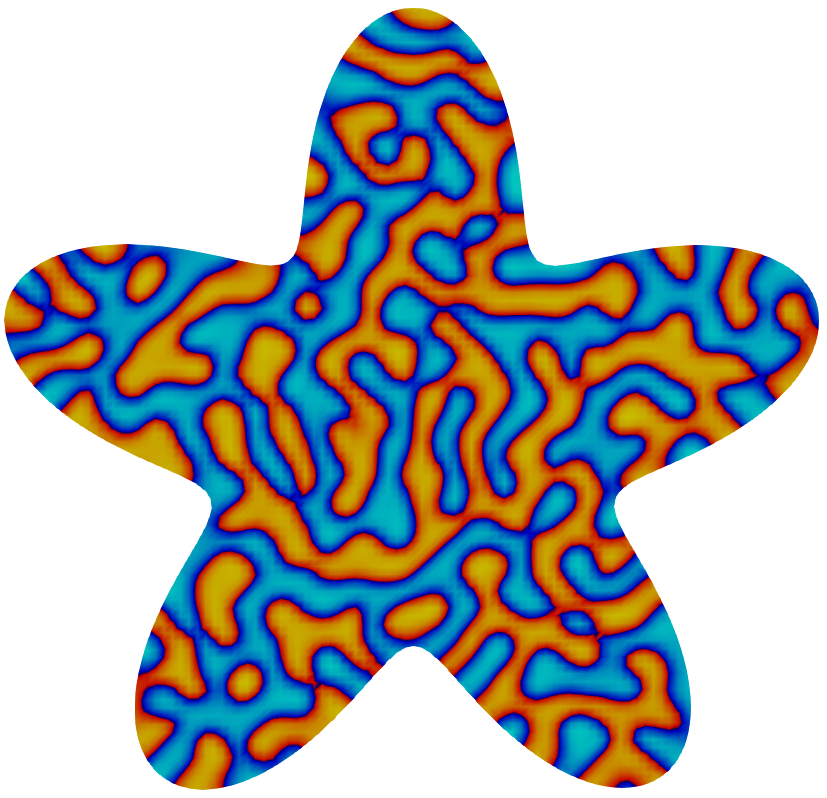
\includegraphics[width=0.3\textwidth]{results/illustration/f50.png}
    }
    \hfill
    \subfloat[$t=200\tau$]{
        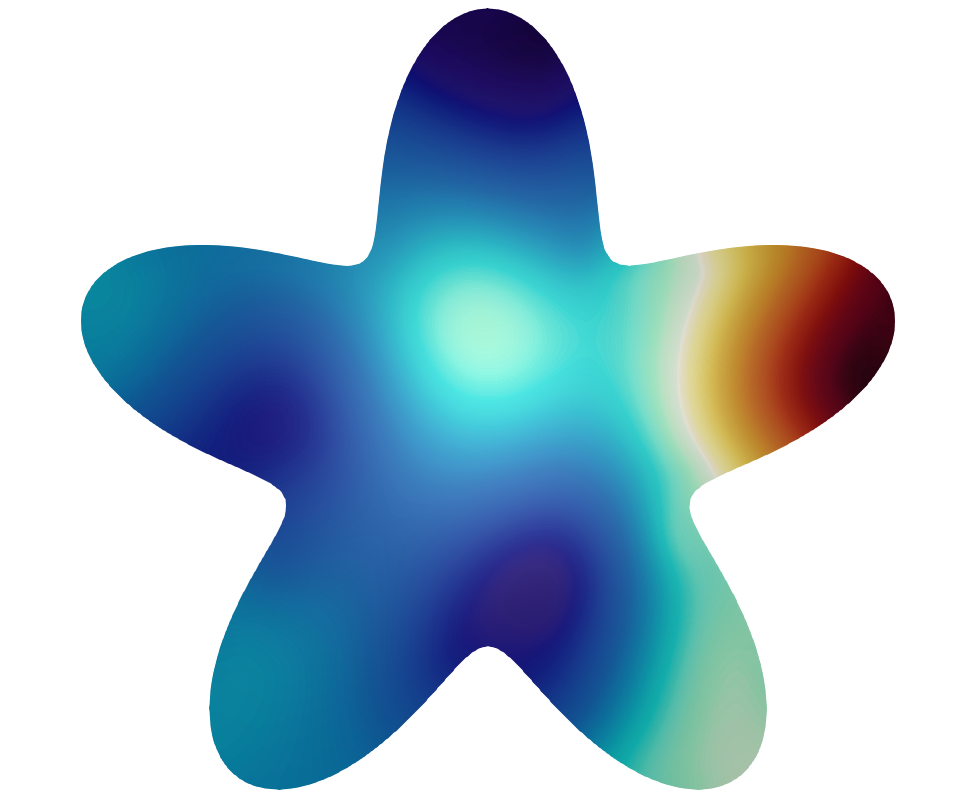
\includegraphics[width=0.3\textwidth]{results/illustration/f200.png}
    }\hfill
    \subfloat[$t=1000\tau$]{
        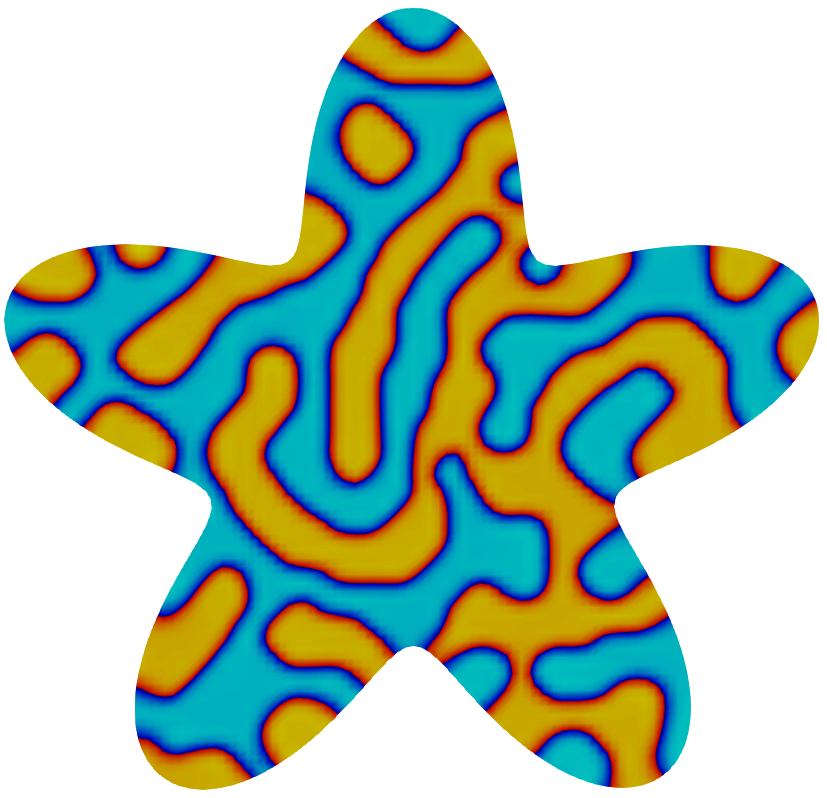
\includegraphics[width=0.3\textwidth]{results/illustration/f500.png}
    }
    \\
    \vspace{10pt}
    \hfill
    \subfloat[$t=50\tau$]{
        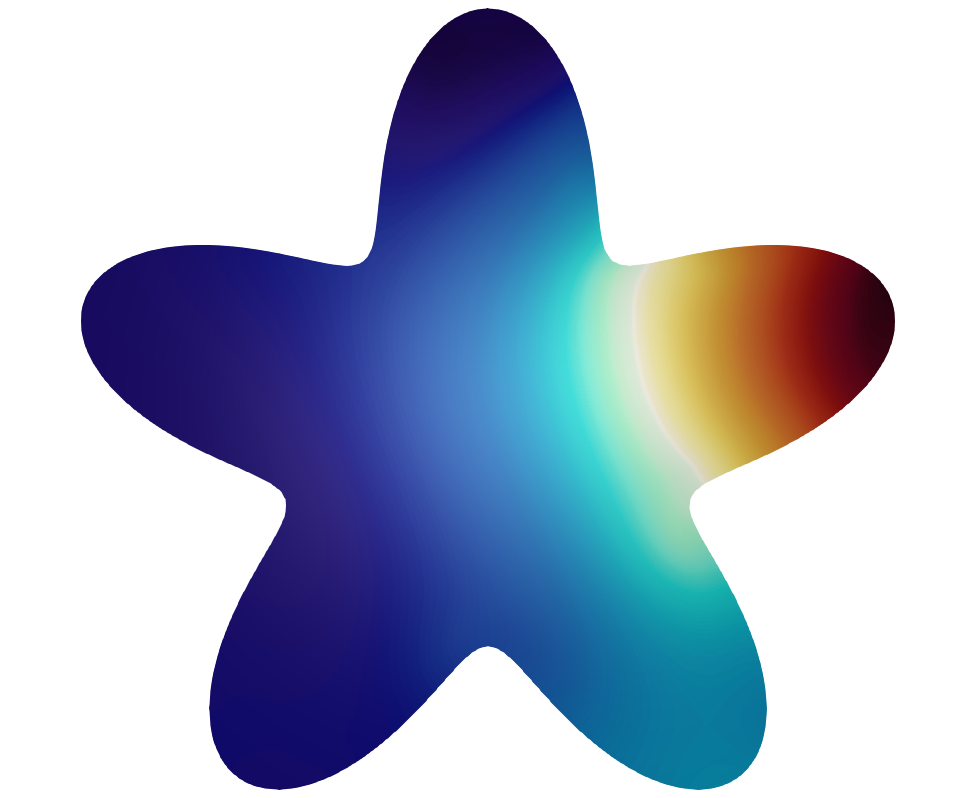
\includegraphics[width=0.3\textwidth]{results/illustration/f1000.png}
    }
    \hfill
    \subfloat[$t=200\tau$]{
        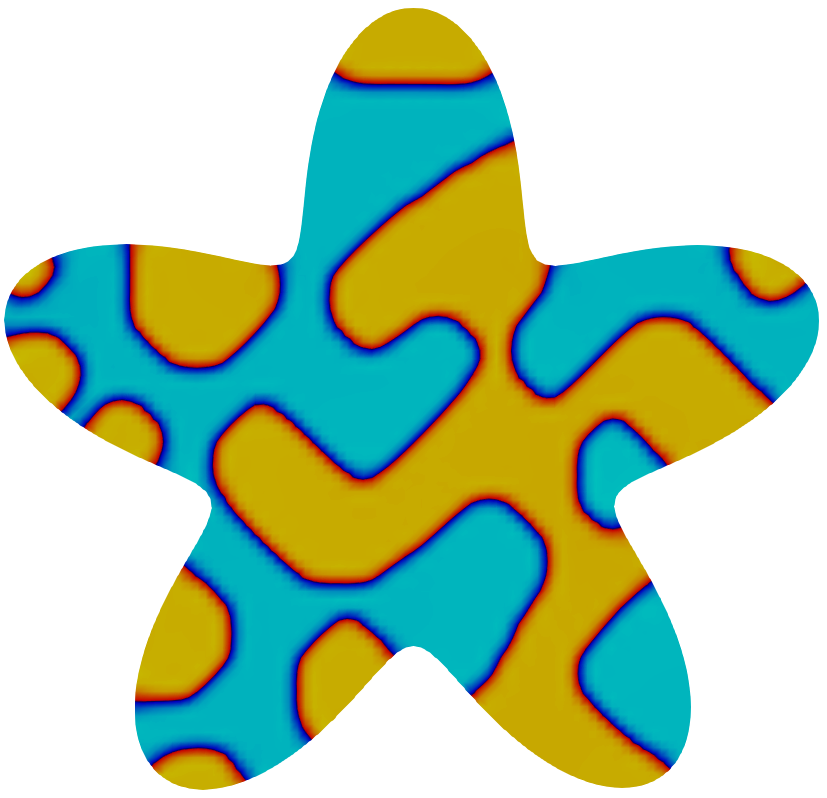
\includegraphics[width=0.3\textwidth]{results/illustration/f5000.png}
    }\hfill
    \subfloat[$t=1000\tau$]{
        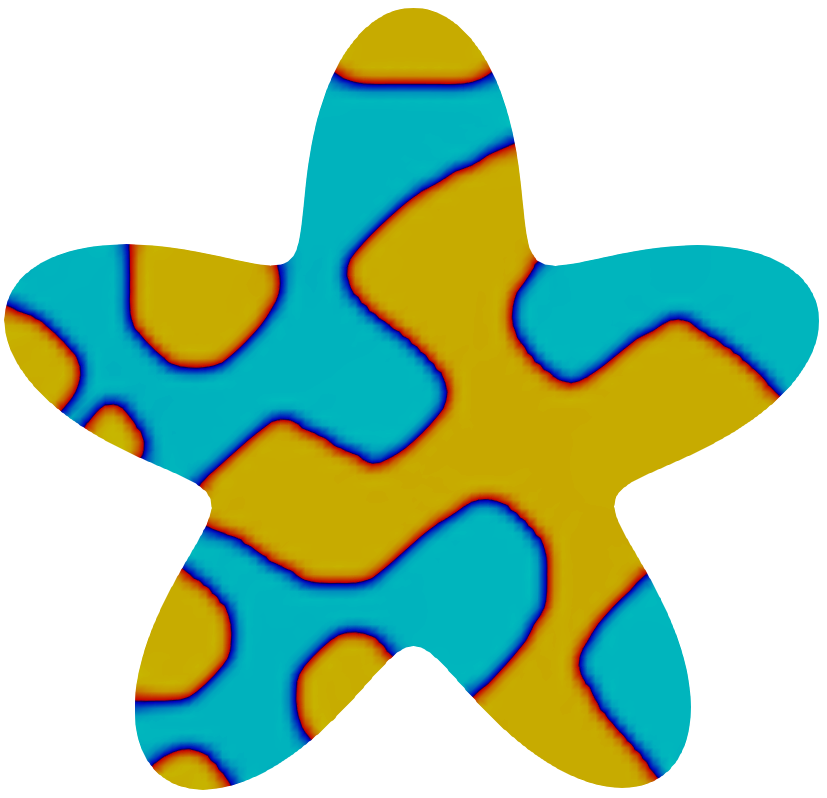
\includegraphics[width=0.3\textwidth]{results/illustration/f10000.png}
    }
    \vspace{10pt}
        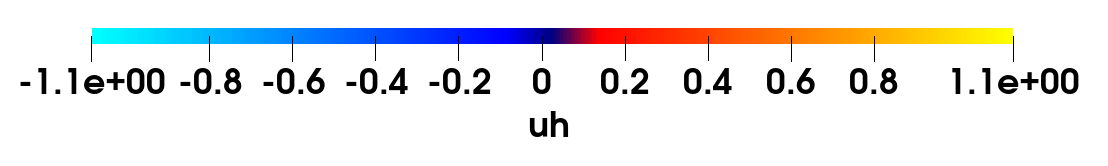
\includegraphics[width=0.8\textwidth]{results/illustration/colobar.png}
    \caption{Illustration of simulations of the Cahn-Hilliard equation on the flower domain for $t\in \left[ 0, 10000\tau  \right] $.}
        \label{sub:fig:ill_flower}
\end{figure}



In our experiments, we defined the initial function $u_{0}(x)$ as the uniform samples from the interval $[-1, 1]$ for each node. That is, for each node $a_{i}$, $u_{0}(a_{i})$ is a sample from the uniform distribution on the interval $[-1, 1]$. This
applies for all $i = 1, \ldots, N$, where $N$ is the total number of degrees of freedom in our system. The node $a_{i}$ is associated with the nodal basis for all $N$ degrees of freedom, as discussed for the discrete system
\eqref{eq:discretized_system}. We again used a square background mesh with length $L=2.7$ and mesh size $h=\frac{L}{n}$ for $n=2^{7}$. For an illustration of the active set $\mathcal{T}_{h} $ (defined in Section \ref{sub:unfitted_mesh}), see Figure \ref{sub:fig:active_mesh}.

\begin{figure}[H]
    \centering
    \hfill
    % \subfloat[]{
        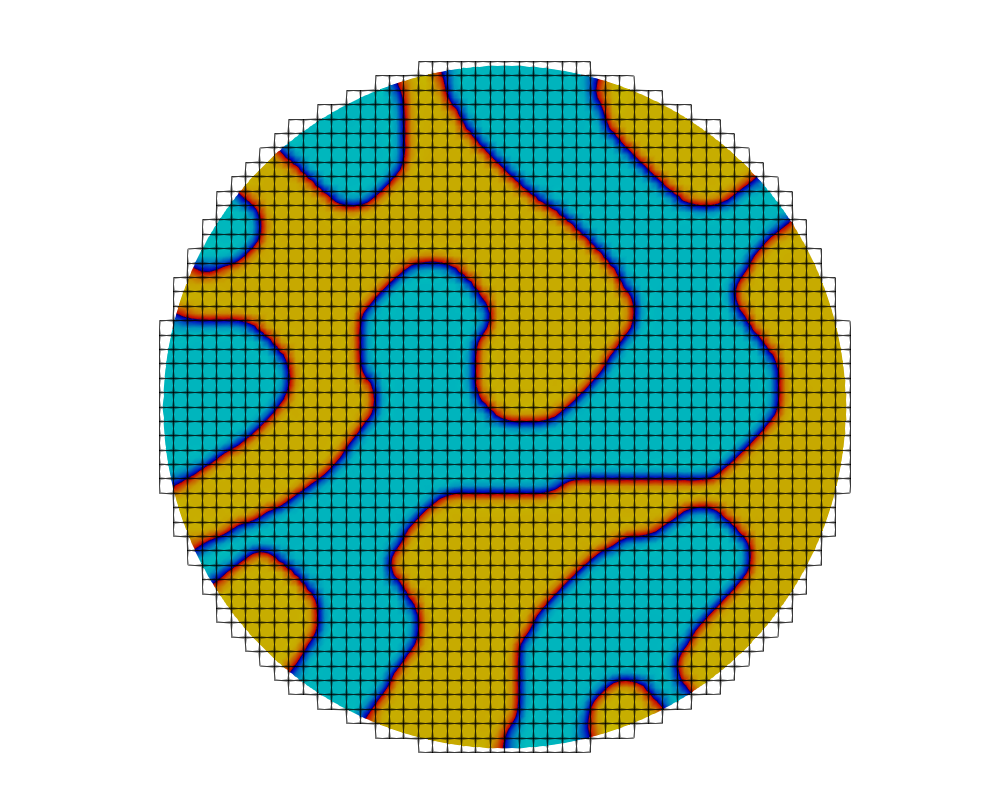
\includegraphics[width=0.45\textwidth]{results/illustration/active_circle.png}
    % }
    \hfill
    % \subfloat[]{
        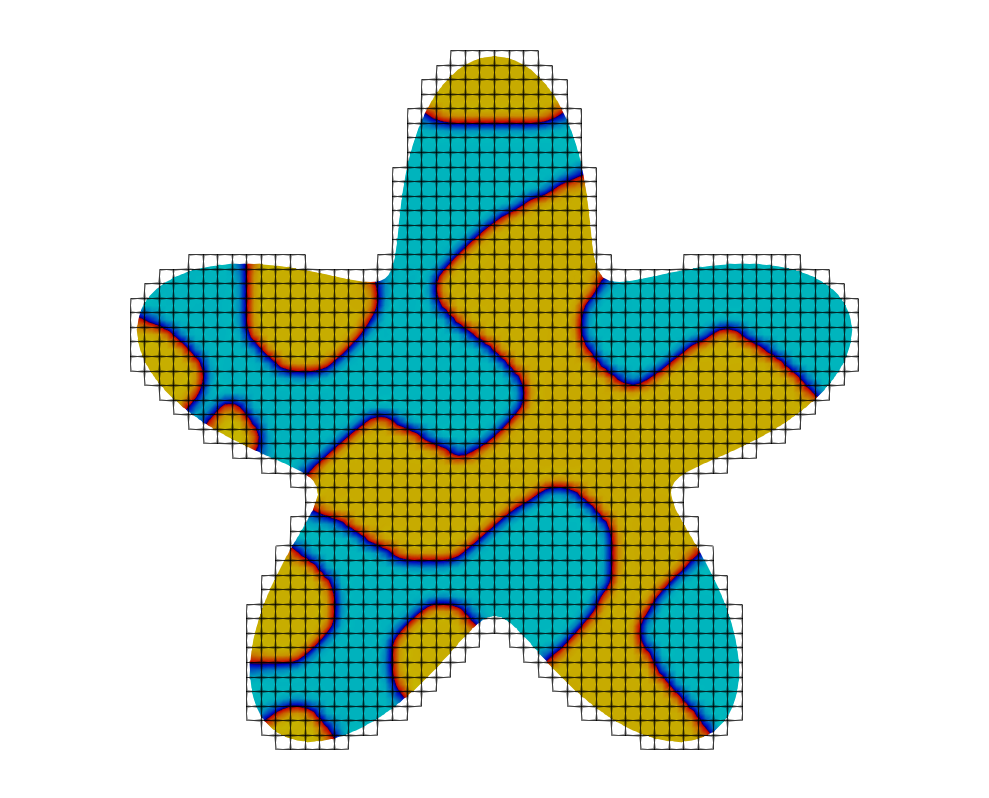
\includegraphics[width=0.45\textwidth]{results/illustration/active_flower.png}
    % }
    \caption{Illustration of the active mesh $\mathcal{T}_{h} $.}
    \label{sub:fig:active_mesh}
\end{figure}


We ran the simulation on the for the flower domain \eqref{eq:flower} and the circular domain \eqref{eq:circle}, illustrated in Figure \ref{sub:fig:ill_flower} and \ref{sub:fig:ill_circle}. The corresponding plots of the mass conservation and energy decrease are presented
in the Figure \ref{fig:physical_CH_plot}, and confirm the expected physical properties of the Cahn-Hilliard equation. The relative error $e_{u}$ shows small deviations of the numerical solution in the order of $10^{ -10 }$ demonstrating that the mass is conserved. We also observe that the energy functional
$E(u_h)$ decreases over time, signifying the system's tendency to seek a state of minimal energy.




\subsection{Note on the manufactured solution}%
\label{sub:the_problem}

While the report is not consisting of a numerical convergence analysis of the Cahn-Hilliard problem, we still present a framework for manufactured solutions for non-homogeneous boundary conditions. Let $ u( x,0) =  u_{0}$ then is Cahn-Hilliard with
non-homogeneous boundary conditions as follows,
\begin{subequations}
    \label{eq:ch_gen}
    \begin{align}
    \label{eq:ch_gen:a}
        \partial _{t} u + \Delta  \left(  \varepsilon^2  \Delta u - f( u) \right)   &= g_{0}( x)   \quad \text{ in } \Omega,  \\
        \partial _{n} u &= g_{1}( x)  \quad \text{ on } \Gamma,  \\
        \partial _{n}    \Delta u   &= g_{2}(x)  \quad \text{ on } \Gamma,
    \end{align}
\end{subequations}
where we defined $f( u) = F'( u) =u( u^2 -1)  $ for $F( u) = \frac{1}{4}( u^{2} - 1)^{2} $ and the domain $\Omega \subset \mathbb{R} ^{d} $  for $d = 2,3$. In contrast to the standard version presented in the introduction \eqref{eq:strongch}, this
version is generalized to also holds for for functions $g_{0},g_{1},g_{2}: \Omega \to\mathbb{R}   $. While the standard version may be physical correct, this version creates flexibility so we can easily construct manufactured solution on complex domains.

    Designing a manufactured solution using $g_{0}( \cdot ) $ may be temping with the formulation \eqref{eq:ch_gen:a}. However, observe that expanding the Laplacian we get,
    \begin{equation}
    \begin{split}
        \Delta  \left(  \varepsilon^2  \Delta u - f( u) \right) & = \varepsilon^2 \Delta^2 u -  \Delta f( u) \\
                                                                                    &= \varepsilon^{2} \Delta ^2 u  - 3( 2u \| \nabla u \|_{ 2 }^{ 2 } + u^{2}  \Delta u )   \\
    \end{split}
    \end{equation}
Here we applied the chain rule twice and inserted the derivatives.
\begin{equation}
    \label{eq:nonlinear_laplace}
    \begin{split}
\Delta f( u)  &= \nabla \cdot \nabla f( u)  = \nabla \cdot  \left[ f' ( u) \partial _{x_{1}}u, \ldots, f' ( u) \partial _{x_{d}}u \right] ^{T} \\
& =  f'' ( u)( ( \partial _{x_{1}}u )^{2} + \ldots +( \partial _{x_{d}}u )^{2} ) +  f' ( u)( \partial _{x_{1} x_{1}}u + \ldots +   \partial _{x_{d} x_{d}}u ) \\
&=  f'' ( u) \| \nabla u \|_{ 2 }^{ 2 } + f' ( u)  \Delta u  = 6u \| \nabla u \|_{ 2 }^{ 2 } + 3u^{2}  \Delta u
    \end{split}
\end{equation}

% Our goal is to write the Cahn Hilliard equation on weak form.
% Assume that $\Omega  \subset \mathbb{R} ^{d}$ with a $\Gamma $ in $C^2$.
%  Let $u \in  H^{4}( \Omega ) $ and $v \in V_{h} $.
% Now, expanding the first Laplace operator from a weak point of view is it clear that
% \[
%  ( \Delta ( \varepsilon  \Delta u - \frac{1}{\varepsilon } f( u) ) ,v )_{\Omega } = \varepsilon ( \Delta^{2} u ,v )_{\Omega } - \frac{1}{\varepsilon } ( \Delta f( u)  ,v )_{\Omega }.
% \]
% Hence, this makes it natural to associate the biharmonic $( \Delta ^2 u,v)_{\Omega } $ with bilinear forms $A_{h}( \cdot ,\cdot ) $ , however, in this section will we only consider the Laplace
% variant $a^{L}( \cdot ,\cdot ) $.
We now seek to find a weak form of the nonlinear term with non homogeneous boundary conditions.
\begin{lemma}[Semi-linear form]
    Let $u \in H^4( \Omega ) $ be solution to \eqref{eq:ch_gen} and $v_{h} \in V_{h}$ the test function.
Then can we rewrite the nonlinear term into the corresponding semi-linear form $c_{h}( \cdot ,\cdot )  $ for the nonlinear term $( -\Delta f( u) , v_{h})_{\Omega }$ into two consistent formulations.
\begin{align}
    \label{eq:ch:1}
      c^{1}_{h} ( u,v_{h})  & = ( f' ( u) \nabla u, \nabla v_{h} )_{\Omega }  - ( f'( u)  g_{1}   ,  v_{h})_{\Gamma } \\
    \label{eq:ch:2}
        c^{2}_{h} ( u,v_{h})  & = -( f( u), \Delta v_{h} )_{\Omega }+  ( f( u) , \jump{ \partial _{n}v_{h} }  )_{\mathcal{F} _{h}^{int}} + ( f(u), \partial _{n} v_{h})_{\Gamma  }  - ( f'( u)  g_{1}   ,  v_{h})_{\Gamma }
\end{align}
% \begin{remark}
%     Be aware that the both formulations are consistent and if we replace $u \in H^{4}( \Omega ) $ with  $u_{h} \in  V_{h}$ we have two different discrete formulations.
% \end{remark}

\end{lemma}
% \todo[inline]{ I criticize \cite[ Remark 4.1d]{feng2007fully} which says that says that finding this weak form is not possible for conforming methods (I guess $C^{0}$ is a conforming method??). }

\begin{proof}

         \textbf{Derivation of \eqref{eq:ch:1}.  }  We want to construct the first formulation. Let $T$ be an element in $\mathcal{T}_{h}$. From Greens theorem is it easy to see that
            \begin{equation}
            \label{eq:1_gr}
-(\Delta f( u) , v_{h})_{T } = (\nabla f( u), \nabla v_{h}  )_{T } - ( \partial _{n}  f( u), v_{h} )_{\partial T }
            \end{equation}
            First by utilizing that $\nabla f( u) = f' ( u) \nabla u $ and $\partial _{n}f( u)  = f' ( u)  \partial _{n}u$  and doing a summation over the triangles  is it clear that \[
            ( -\Delta f( u),v_{h} )_{\Omega  } =(f' ( u) \nabla u, \nabla v_{h}  )_{\Omega  } - (   f' ( u)\partial _{n}u, v_{h} )_{\partial \mathcal{T}_{h}  }
            \]
            Iterating over the facets is it clear that \[
                \begin{split}
            (   f' ( u)\partial _{n}u, v_{h} )_{\partial \mathcal{T}_{h}  } & = \sum_{F \in \mathcal{F}_{h}  }^{} \int_{F}^{}   \jump{ f' ( u)\partial _{n}u, v_{h} } \\
                                                                        & =  ( \jump{ f' ( u) \partial _{n}u },  \mean{v_{h}}    )_{\mathcal{F}^{int}_{h} } + ( \mean{ f' ( u) \partial _{n}u }, \jump{ v_{h} }    )_{\mathcal{F}^{int}_{h} } +  ( f' ( u)
                                                                        \partial _{n}u, v_{h}) _{\Gamma } \\
                                                                        & =  ( f' ( u) \partial _{n}u, v_{h}) _{\Gamma }
                \end{split}
            \]
            The jump terms vanishes by the regularity of $u$ and $v_{h}$. Hence, by inserting $g_{1}$ we have shown that the first formulation holds.

         \textbf{Derivation of \eqref{eq:ch:2}.  }  Applying a extra iteration of Greens theorem on \eqref{eq:1_gr} we get the following terms.
\[
    \begin{split}
-(\Delta f( u) , v_{h})_{T }  = -( f( u), \Delta v_{h} )_{T} + (f( u), \partial _{n} v_{h}  )_{\partial T} - (   f'( u)\partial _{n}u, v_{h} )_{\partial T } .
    \end{split}
\]
Now, by doing a summation of all triangles it is clear that this holds.
\begin{equation}
\label{eq:f_g2}
-(\Delta f( u) , v_{h})_{\Omega  }  = -( f( u), \Delta v_{h} )_{\Omega } + (f( u), \partial _{n} v_{h}  )_{\partial \mathcal{T}_{h} } - (   f'( u)\partial _{n}u, v_{h} )_{\partial \mathcal{T}_{h}  }
\end{equation}
It comes evident from the first step of the proof that $ (   f'( u)\partial _{n}u, v_{h} )_{\partial \mathcal{T}_{h}  } = (   f'( u)\partial _{n}u, v_{h} )_{\Gamma }$, hence, we only need to compute the term $(f( u), \partial _{n} v_{h}  )_{\partial
\mathcal{T}_{h} }$ on the facets. \[
    \begin{split}
(f( u), \partial _{n} v_{h}  )_{\partial
\mathcal{T}_{h} } & = \sum_{F\in \mathcal{F} _{h}}^{} \int_{F}^{}\jump{ f( u), \partial _{n} v_{h}  } \\
& =  (\jump{ f( u)  }  , \mean{ \partial _{n} v_{h} }    )_{ \mathcal{F}_{h}^{int} } +(\mean{ f( u)  }  , \jump{ \partial _{n} v_{h} }    )_{ \mathcal{F}_{h}^{int} } + (f( u), \partial _{n} v_{h}  )_{\Gamma } \\
&=  (\mean{ f( u)  }  , \jump{ \partial _{n} v_{h} }    )_{ \mathcal{F}_{h}^{int} } + (f( u), \partial _{n} v_{h}  )_{\Gamma }
    \end{split}
\]
Again one of the jump terms vanishes because of the regularity of $u$.
Inserting the result into \eqref{eq:f_g2} have we shown that the second formulation also holds.
\end{proof}


Combining the full general Cahn-Hilliard problem in \eqref{eq:ch_gen} with the semi-linear forms\eqref{eq:ch:1} and the CutCIP biharmonic problem \eqref{eq:discrete_CutCIP_prob}, we get the following scheme.
\begin{equation}
    ( \partial _{t}u_{h}, v_{h})_\Omega + \varepsilon^2  A_{h}( u_{h},v_{h}) + c_{h}( u_{h},v_{h})   =   l_{h}(v_{h}) \quad  \forall u_{h}, v_{h} \in V_{h}
\end{equation}

To illustrate, assume we use the Laplace formulation presented in \eqref{eq:laplace_prob} integrated into \eqref{eq:discrete_CutCIP_prob}, i.e. $A_{h}( u_{h}, v_{h}) = a^{L}_{h}( u_{h}, v_{h}) + g_{h}( u_{h}, v_{h})   = l_{h}^{L}( v_{h})$. Due to the $\varepsilon $ scaling, we ultimately
arrive at the following modification.
 \begin{equation}
    l_{h}^{L}( v_{h})  =  \left( g_{0}, v_{h} \right) _{\Omega } -  \varepsilon^2 ( g_{2},  v_{h} )_{\Gamma }  -  \varepsilon^2 ( g_{1}, \Delta  v_{h}  )_{\Gamma }  + \varepsilon^2 \frac{\gamma }{h} ( g_{1}, \partial _{n} v_{h}  )_{\Gamma }
 \end{equation}
 Hence, we arrived at a system which can easily be used to construct manufactured solution.

